\documentclass[border=7pt]{standalone}
\usepackage{amsmath}
\usepackage{mathptmx}
\usepackage{tikz}
\usetikzlibrary{arrows.meta,shadows}

\definecolor{ink}{HTML}{3A3936}
\definecolor{muted}{HTML}{656461}
\definecolor{dataF}{HTML}{F0EFEC}
\definecolor{modelE}{HTML}{2A78D6}\definecolor{modelF}{HTML}{DCE9F9}
\definecolor{augE}{HTML}{EB6834}\definecolor{augF}{HTML}{FDE3D6}
\definecolor{opE}{HTML}{6250D6}\definecolor{opF}{HTML}{EBE9FB}
\definecolor{lossE}{HTML}{1BAF7A}\definecolor{lossF}{HTML}{D9F3E9}

\tikzset{
  every node/.style={font=\small,text=ink,align=center},
  base/.style={rectangle,rounded corners=3pt,minimum height=12mm,inner sep=3pt,line width=0.8pt},
  data/.style={base,fill=dataF,draw=muted,text width=23mm},
  model/.style={base,fill=modelF,draw=modelE,text width=25mm},
  aug/.style={base,fill=augF,draw=augE,line width=1.2pt,text width=24mm},
  target/.style={base,fill=opF,draw=opE,text width=42mm},
  loss/.style={base,fill=lossF,draw=lossE,text width=30mm},
  tensor/.style={rectangle,fill=white,draw=modelE,line width=.8pt,minimum width=7mm,minimum height=9mm,
    double copy shadow={shadow xshift=1.5pt,shadow yshift=1.5pt,draw=modelE,fill=white}},
  flow/.style={-{Stealth[length=2.3mm]},line width=.8pt,draw=ink,rounded corners=4pt},
  fixed/.style={flow,densely dashed,draw=opE},
  note/.style={font=\footnotesize\itshape,text=muted},
}
\newcommand{\sub}{\footnotesize\color{muted}}

\begin{document}
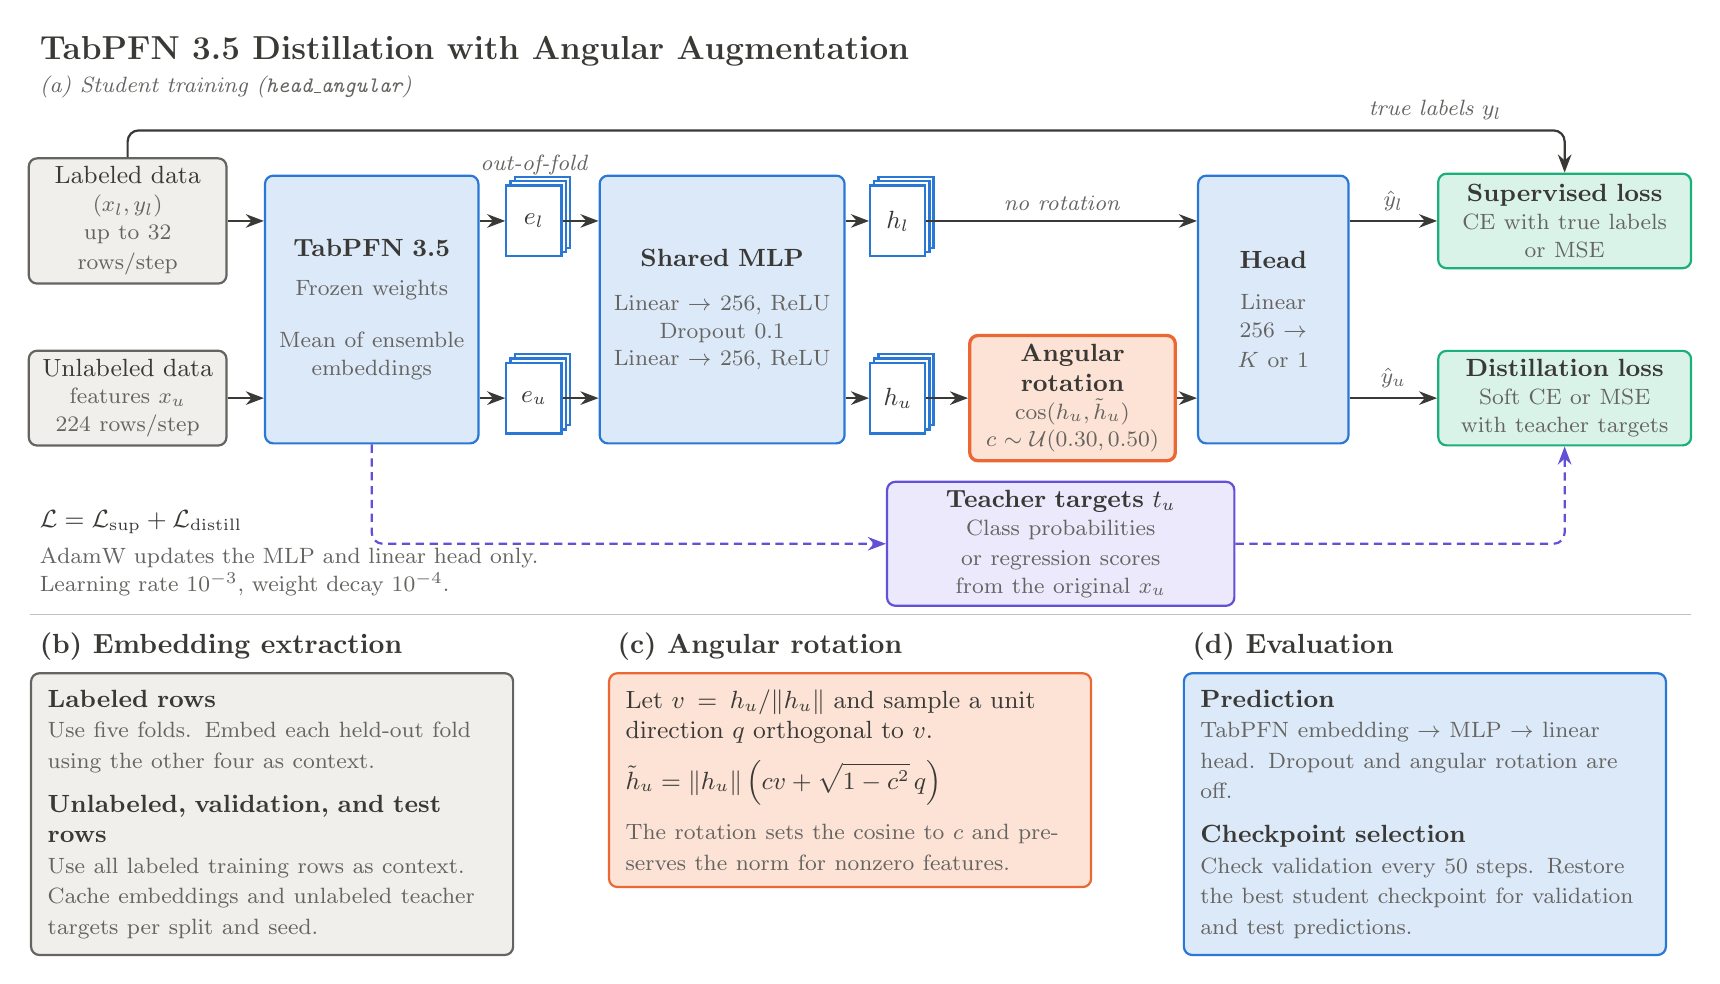
\begin{tikzpicture}
\def\yU{-2.25}
\def\yTeacher{-4.1}

\node[anchor=west,font=\large\bfseries] at (-1.24,2.15) {TabPFN 3.5 Distillation with Angular Augmentation};
\node[note,anchor=west] at (-1.24,1.70) {(a) Student training (\texttt{head\_angular})};

\node[data] (xl) at (0,0) {Labeled data\\[-1pt]{\sub $(x_l,y_l)$}\\[-1pt]{\sub up to 32 rows/step}};
\node[data] (xu) at (0,\yU) {Unlabeled data\\[-1pt]{\sub features $x_u$}\\[-1pt]{\sub 224 rows/step}};
\node[model,minimum height=34mm] (pfn) at (3.1,-1.125)
  {\textbf{TabPFN 3.5}\\[3pt]{\sub Frozen weights}\\[8pt]{\sub Mean of ensemble}\\[-1pt]{\sub embeddings}};
\node[tensor] (el) at (5.16,0) {$e_l$};
\node[tensor] (eu) at (5.16,\yU) {$e_u$};
\node[note,above] at (el.north) {out-of-fold};

\node[model,text width=29mm,minimum height=34mm] (mlp) at (7.55,-1.125)
  {\textbf{Shared MLP}\\[5pt]{\sub Linear $\to$ 256, ReLU}\\[-1pt]{\sub Dropout 0.1}\\[-1pt]{\sub Linear $\to$ 256, ReLU}};
\node[tensor] (hl) at (9.78,0) {$h_l$};
\node[tensor] (hu) at (9.78,\yU) {$h_u$};
\node[aug] (angular) at (12.00,\yU)
  {\textbf{Angular rotation}\\[-1pt]{\sub $\cos(h_u,\tilde h_u)$}\\[-1pt]{\sub $c\sim\mathcal{U}(0.30,0.50)$}};
\node[model,text width=17mm,minimum height=34mm] (head) at (14.55,-1.125)
  {\textbf{Head}\\[4pt]{\sub Linear}\\[-1pt]{\sub 256 $\to$ $K$ or $1$}};

\node[loss] (sup) at (18.25,0) {\textbf{Supervised loss}\\[-1pt]{\sub CE with true labels}\\[-1pt]{\sub or MSE}};
\node[loss] (dist) at (18.25,\yU) {\textbf{Distillation loss}\\[-1pt]{\sub Soft CE or MSE}\\[-1pt]{\sub with teacher targets}};
\node[target] (teacher) at (11.85,\yTeacher)
  {\textbf{Teacher targets $t_u$}\\[-1pt]{\sub Class probabilities or regression scores}\\[-1pt]{\sub from the original $x_u$}};

\draw[flow] (xl.east) -- (xl -| pfn.west);
\draw[flow] (xu.east) -- (xu -| pfn.west);
\draw[flow] (pfn.east |- el) -- (el.west);
\draw[flow] (pfn.east |- eu) -- (eu.west);
\draw[flow] (el.east) -- (el -| mlp.west);
\draw[flow] (eu.east) -- (eu -| mlp.west);
\draw[flow] (mlp.east |- hl) -- (hl.west);
\draw[flow] (mlp.east |- hu) -- (hu.west);
\draw[flow] (hl.east) -- node[note,above] {no rotation} (hl -| head.west);
\draw[flow] (hu.east) -- (angular.west);
\draw[flow] (angular.east) -- (angular -| head.west);
\draw[flow] (head.east |- sup) -- node[note,above] {$\hat y_l$} (sup.west);
\draw[flow] (head.east |- dist) -- node[note,above] {$\hat y_u$} (dist.west);
\draw[flow] (xl.north) -- (0,1.15) -- node[note,above,pos=.91] {true labels $y_l$} (18.25,1.15) -- (sup.north);
\draw[fixed] (pfn.south) |- (teacher.west);
\draw[fixed] (teacher.east) -| (dist.south);


\node[anchor=west,align=left] at (-1.24,-4.22)
  {$\mathcal L=\mathcal L_{\mathrm{sup}}+\mathcal L_{\mathrm{distill}}$\\[2pt]
   {\sub AdamW updates the MLP and linear head only.}\\[-1pt]
   {\sub Learning rate $10^{-3}$, weight decay $10^{-4}$.}};

\draw[muted!40,line width=.6pt] (-1.24,-5.0) -- (19.86,-5.0);

\node[anchor=west,font=\normalsize\bfseries] at (-1.24,-5.40) {(b) Embedding extraction};
\node[anchor=west,font=\normalsize\bfseries] at (6.10,-5.40) {(c) Angular rotation};
\node[anchor=west,font=\normalsize\bfseries] at (13.40,-5.40) {(d) Evaluation};

\node[base,fill=dataF,draw=muted,anchor=north west,text width=57mm,align=left,inner sep=6pt]
  at (-1.24,-5.73) {\textbf{Labeled rows}\\
    {\sub Use five folds. Embed each held-out fold using the other four as context.}\\[5pt]
    \textbf{Unlabeled, validation, and test rows}\\
    {\sub Use all labeled training rows as context. Cache embeddings and unlabeled teacher targets per split and seed.}};

\node[base,fill=augF,draw=augE,anchor=north west,text width=57mm,align=left,inner sep=6pt]
  at (6.10,-5.73) {Let $v=h_u/\lVert h_u\rVert$ and sample a unit direction $q$ orthogonal to $v$.\\[5pt]
    $\displaystyle \tilde h_u=\lVert h_u\rVert\left(cv+\sqrt{1-c^2}\,q\right)$\\[6pt]
    {\sub The rotation sets the cosine to $c$ and preserves the norm for nonzero features.}};

\node[base,fill=modelF,draw=modelE,anchor=north west,text width=57mm,align=left,inner sep=6pt]
  at (13.40,-5.73) {\textbf{Prediction}\\
    {\sub TabPFN embedding $\to$ MLP $\to$ linear head. Dropout and angular rotation are off.}\\[5pt]
    \textbf{Checkpoint selection}\\
    {\sub Check validation every 50 steps. Restore the best student checkpoint for validation and test predictions.}};
\end{tikzpicture}
\end{document}
